\documentclass[a4paper]{article}

\usepackage{fullpage}
\usepackage{hyperref}
\usepackage{graphicx}
\usepackage[T1]{fontenc}


\title{Ex2Gr}
\author{Manuel d'utilisation, année 2020-2021}
\date{Loïg Jezequel}

\begin{document}

\maketitle{}

Ex2Gr (exercices de graphes) est un logiciel permettant de faire des exercices de base sur le vocabulaire et les notions fondamentales sur les graphes vues dans le cours M2201 - graphes et langages à l'IUT d'informatique de Nantes.
Le présent manuel d'utilisation explique comment installer et utiliser Ex2Gr.

\section*{Récupérer Ex2Gr}

Ex2Gr est disponible sur la page Madoc du module ainsi que sur Github à l'adresse suivante~: \url{https://github.com/loig/ex2gr} (où est aussi disponible le code du programme, sous licence GNU GPLv3).
Des exécutables sont fournis pour les systèmes Windows et Linux.
Il est possible, simplement, de produire un exécutable pour un système MacOS en clonant le répertoire et en utilisant la commande \verb|go build| (à condition d'avoir Go sur sa machine).

\section*{Démarrer Ex2Gr}

\paragraph{Systèmes Linux.} Il faudra rendre le fichier récupéré exécutable (\verb|chmod u+x ex2gr|) puis le lancer à l'aide d'un terminal.

\paragraph{Systèmes Windows.} On peut simplement double-cliquer sur le fichier récupéré pour le lancer. Cependant, il est recommandé de lancer le programme dans un terminal (des informations utiles sont affichées sur la sortie standard).

\section*{Utiliser Ex2Gr}

\paragraph{Écran de sélection des exercices.}
Au lancement, une fenêtre s'ouvre (fig.~\ref{fig:welcomescreen}).
Chaque carré représente un exercice.
Sur la figure la souris est sur le troisième exercice de la première ligne.
En bas de la fenêtre le titre de cet exercice s'affiche, ainsi que quelques autres informations (nombre de tentatives effectuées, exercice déjà fait ou pas).
Pour démarrer l'exercice il suffit de faire un clic gauche.
Enfin, en cliquant (clic gauche toujours) sur le bouton «Sauvegarder et quitter» on quitte le logiciel et les progrès sont sauvegardés dans un fichier \verb|ex2grSave.json|.

\paragraph{Écran de réponse à un exercice.}
Une fois un exercice sélectionné, on arrive sur un écran qui se présente comme sur la figure~\ref{fig:exo}.
Pour la plupart des exercices, il suffit de cliquer (clic gauche) sur l'une des réponse proposées pour répondre à l'exercice.
Pour une partie d'entre-eux il faut modifier un graphe (sous différentes formes, voir la partie suivante à ce propos).
Chaque exercice demande de répondre correctement à cinq questions d'affilée (sans sortir de l'exercice), sous le titre de l'exercice les progrès sont indiqués (ici l'utilisateur a répondu pour le moment à deux questions d'affilée).
En haut à droite se trouve un bouton qui permet de quitter l'exercice en cours (attention, si vous le faites vous perdez votre avancée sur l'exercice).
En haut à gauche se trouve un code qui permettra à vos enseignants de retrouver la question exacte sur laquelle vous travaillez : si vous avez des questions il faut leur transmettre ce code.
Pour vous simplifier la vie, si vous avez lancé Ex2Gr depuis un terminal, ce code s'affiche aussi dans celui-ci, ce qui vous permet de le copier-coller.

\paragraph{Options au lancement.}
Au lancement de Ex2Gr vous pouvez éventuellement préciser deux options~: \verb|-sauvegarde monFichier| pour sauvegarder/récupérer vos progrès depuis le fichier \verb|monFichier| plutôt que depuis le fichier par défaut \verb|ex2grSave.json| (si le fichier n'existe pas il est créé, si le fichier existe mais ne contient pas des données formatées comme il faut le logiciel risque de planter) et \verb|-seed code| où \verb|code| est le code d'une question (visible en haut à gauche et dans le terminal) pour afficher une question donnée (ceci permettra surtout à vos enseignants de voir ce sur quoi vous travaillez quand vous leur posez des questions).

\section*{Modifier des graphes}

Dans toutes les questions, vous pouvez passer votre souris au dessus des différentes représentations des graphes pour visualiser plus simplement certaines choses (sommets, arcs, lignes et colonnes des matrices, etc).

\paragraph{Représentation visuelle.} Dans la représentation visuelle des graphes vous pouvez toujours déplacer les sommets en faisant un glisser/déposer avec le bouton droit de votre souris.
De même, vous pouvez toujours déplacer les boucles autour d'un sommet en cliquant (clic droit) simplement dessus.
Dans les exercices qui le demandent vous pouvez modifier les graphes en maintenant le clic gauche de la souris pour tirer des arcs d'un sommet à un autre.
Dans ces exercices vous pouvez aussi supprimer des arcs en cliquant (clic gauche) dessus.

\paragraph{Représentation matricielle.} Dans les exercices qui demandent de modifier la représentation en matrice d'adjacence d'un graphe, vous pouvez modifier le contenu d'une case (0 ou 1) simplement en cliquant dessus (clic gauche).

\paragraph{Représentation en listes de successeurs.} Dans les exercices qui demandent de modifier des listes de successeurs vous pouvez ajouter un élément dans une liste en cliquant (clic gauche) sur le symbole \verb|+| à droite de cette liste, retirer un élément (celui de droite) en cliquant (clic gauche) sur le symbole \verb|-| à droite de cette liste, modifier un élément en cliquant (clic gauche) dessus (le remplace par le prochain sommet qui n'apparaît pas encore dans la liste).

\section*{Signaler des bugs}

Ex2Gr a été développé assez rapidement pour vous permettre de vous exercer sur les graphes à distance.
Si vous regardez le code, vous verrez qu'il n'est pas très propre.
Il est donc très possible qu'il y ait quelques bugs.
Si vous pensez en avoir détecté un, n'hésitez pas à m'en faire part (par exemple par mail à l'adresse \url{loig.jezequel@univ-nantes.fr}) au plus vite pour que je puisse corriger cela pour les étudiants qui n'ont pas encore eu leur TD.

De même, si vous pensez qu'il manque des informations dans cette documentation, vous pouvez me contacter.
Je la mettrai à jour si besoin.

\begin{figure}[htbp]
  \centering
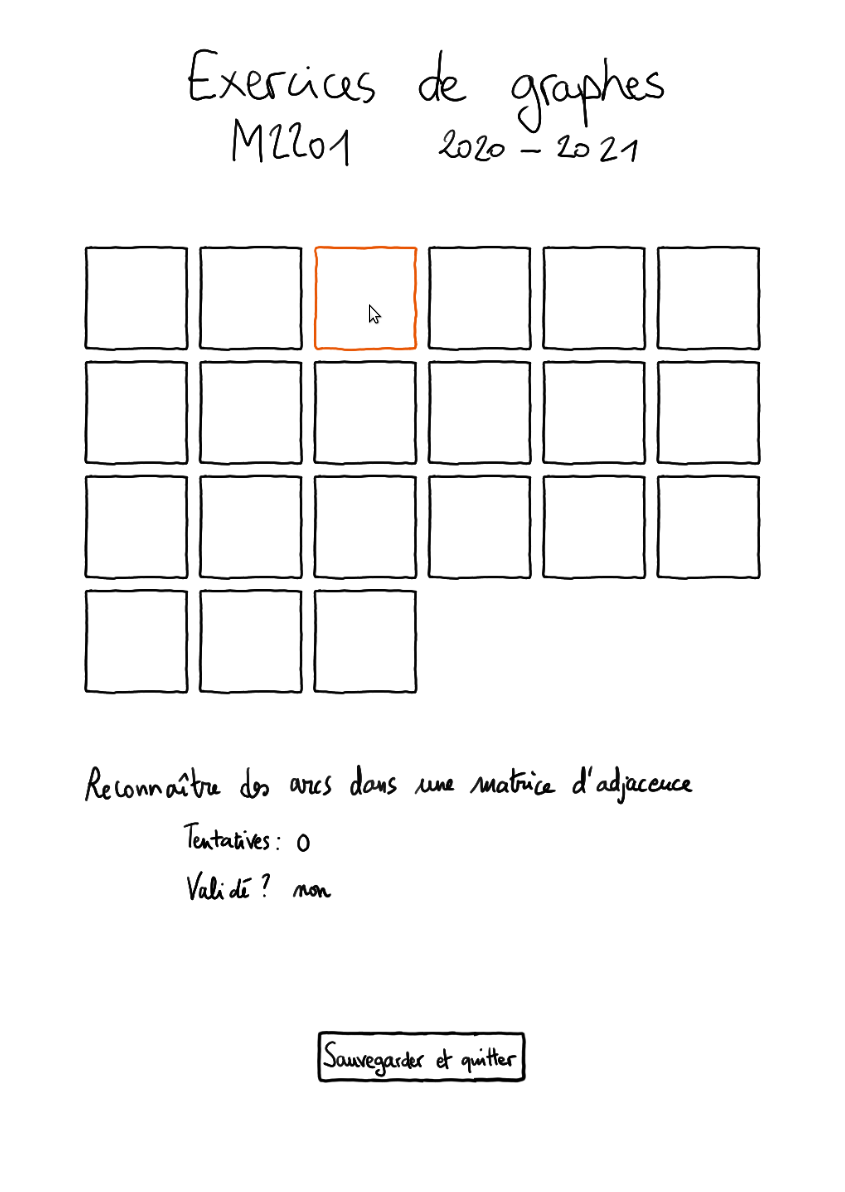
\includegraphics[width=12cm]{welcome.png}
\caption{Écran d'accueil de Ex2Gr}\label{fig:welcomescreen}
\end{figure}

\begin{figure}[htbp]
  \centering
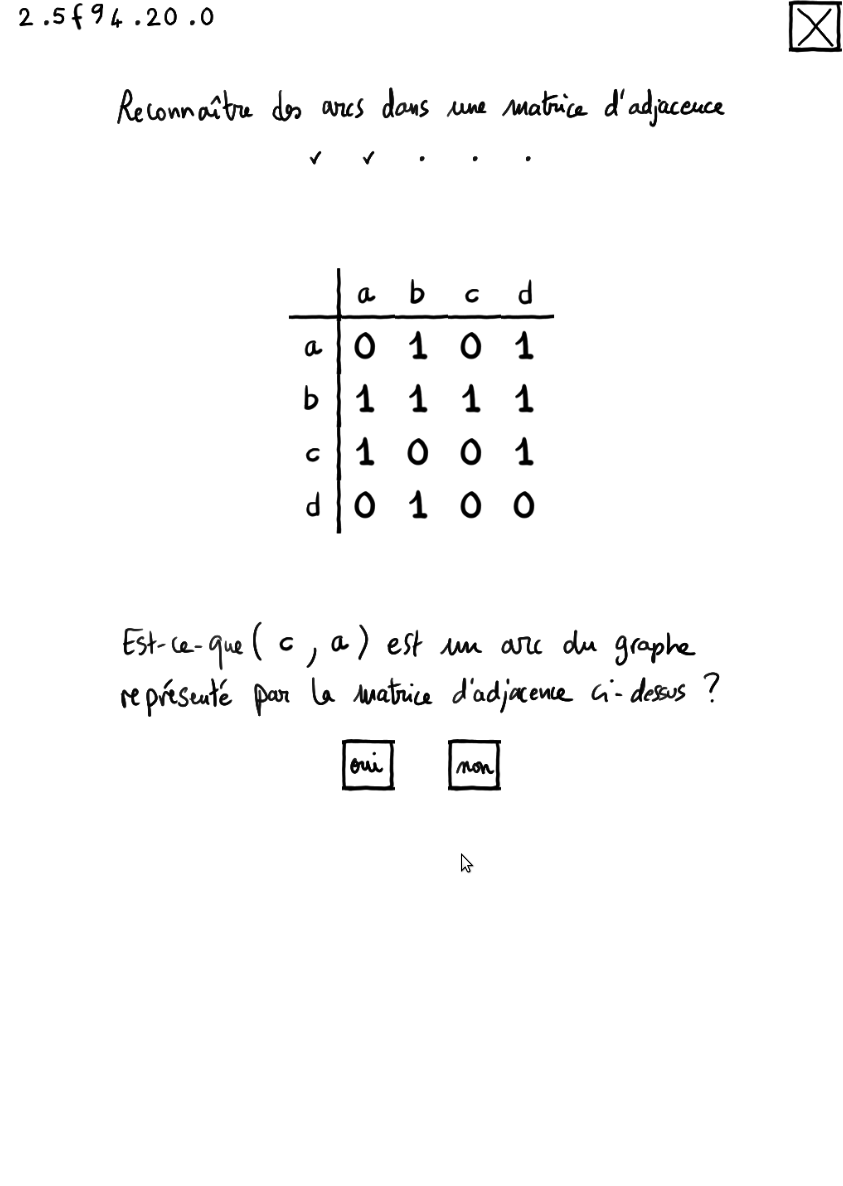
\includegraphics[width=12cm]{exo.png}
\caption{Écran de réponse à un exercice de Ex2Gr}\label{fig:exo}
\end{figure}



\end{document}
